%% SN Computer Science (Springer Nature) submission, Review Article.
%% Built on the Springer Nature LaTeX template (sn-jnl.cls): open "Springer Nature LaTeX Template" on Overleaf,
%% replace its sample .tex with this file, upload refs.bib, compile with pdfLaTeX + BibTeX. See SUBMISSION.md.
\documentclass[pdflatex,sn-mathphys-num]{sn-jnl}% numbered references

\usepackage{graphicx}
\usepackage{multirow}
\usepackage{amsmath,amssymb,amsfonts}
\usepackage{array}
\usepackage{booktabs}
\usepackage{xcolor}
\usepackage{tikz}
\usetikzlibrary{arrows.meta,positioning,calc,fit}
\newcolumntype{L}[1]{>{\raggedright\arraybackslash}p{#1}}

\raggedbottom

\begin{document}

\title[Agentic Retrieval-Augmented Generation: A Survey]{From Retrieve-Then-Read to Learned Search Policies: A Survey of Agentic Retrieval-Augmented Generation}

\author*[1]{\fnm{Swapnali} \sur{Gaikwad}}\email{swapnali.gaikwad@dypvp.edu.in}
\author[1]{\fnm{Ajit} \sur{Paraskar}}\email{ajitparaskar87@gmail.com}
\author[1]{\fnm{Prathamesh} \sur{Kumbhar}}\email{prathameshkumbhar.dev@gmail.com}
\author[1]{\fnm{Harshvardhan} \sur{Patil}}\email{harsh.patil.tech@gmail.com}
\author[1]{\fnm{Bikram} \sur{Ghosh}}\email{ghoshbikram2725@gmail.com}

\affil[1]{\orgdiv{Department of Computer Engineering}, \orgname{Dr. D. Y. Patil Institute of Technology}, \orgaddress{\city{Pimpri, Pune}, \postcode{411018}, \state{Maharashtra}, \country{India}}}

\abstract{Retrieval-augmented generation (RAG) lets a large language model answer from documents it was never trained on. The classic recipe retrieves once and then reads, and it breaks down on questions that need several hops, on noisy or misleading passages, and on data that changes. Agentic RAG hands the model control over retrieval: it may split the question, search more than once, choose among tools, decide how much text to read, check its own answer and remember what it learned. This survey reviews that line of work. We cast agentic RAG as a sequential decision problem and use the decisions it exposes to organise the literature into eight dimensions: query planning, iterative retrieval, search policy and evidence granularity, self-verification, tool use, long-term memory, attribution, and evaluation. We compare 25 representative methods along these dimensions, examine in detail the GRASP policy, which learns at each step whether to search semantically, search by keyword or read a whole paragraph, and review benchmarks and attacks specific to retrieval agents. Three patterns stand out. Reinforcement-learned search policies are trained and tested almost entirely on static Wikipedia corpora with gold evidence; verification, memory and actions are studied apart from learned retrieval; and no public benchmark scores an agent that answers from private, changing, multi-source data and also acts on it. We close with open problems that follow from these gaps.}

\keywords{Retrieval-augmented generation, Agentic RAG, Large language models, Search policy, Citation verification, Agent memory}

\maketitle

%=====================================================================
\section{Introduction}
\label{sec:intro}
%=====================================================================

A language model knows what was in its training data and nothing after it. Retrieval-augmented generation (RAG) fixes part of this by fetching passages from an external collection and conditioning the answer on them~\cite{lewis2020rag,guu2020realm}. In its common form a retriever ranks chunks once and a generator reads the top few~\cite{gao2023ragsurvey,fan2024ragsurvey}. The approach works well when one passage holds the answer and the collection does not change. It works badly in three other situations. Some questions can only be searched in steps, because the second half names an entity that the first half has to find~\cite{trivedi2023ircot,press2023selfask}. Retrieved text can be wrong or off-topic, and models are easily distracted by it~\cite{shi2023distracted,liu2024lost}. And some facts, such as deadlines and prices, keep changing~\cite{vu2024freshllms}.

Agentic RAG moves these decisions into the model. The model chooses whether to decompose the question, when to search and with which tool, how much of a result to read, whether its evidence is enough, and what to keep for later~\cite{singh2025agenticrag}. The first systems did this through prompting~\cite{yao2023react,trivedi2023ircot,jiang2023flare}. Since early 2025 a growing set of methods trains the search behaviour with reinforcement learning (RL), rewarding only the final answer or a few auxiliary signals~\cite{jin2025searchr1,song2025r1searcher,chen2025research,zheng2025deepresearcher}.

Several surveys already cover parts of this ground. Gao \textit{et al.} trace RAG from naive through advanced to modular pipelines~\cite{gao2023ragsurvey}. Fan \textit{et al.} organise retrieval-augmented LLMs by architecture, training strategy and application~\cite{fan2024ragsurvey}. Singh \textit{et al.} classify agentic RAG by agent architecture~\cite{singh2025agenticrag}, and Wang \textit{et al.} survey LLM agents in general~\cite{wang2024agentsurvey}. Table~\ref{tab:surveys} sets these against the present work. None of them covers the 2025--2026 wave of RL-trained search policies, and none treats evidence granularity, that is, how much text an agent chooses to read, as a decision in its own right.

\begin{table}[t]
\centering
\caption{Related surveys and what each covers. A check means the topic is treated in some depth; a dash means it is absent or mentioned only in passing.}
\label{tab:surveys}
\footnotesize
\begin{tabular}{@{}lccccc@{}}
\toprule
Survey & RAG & Agents & RL search & Granularity & Security \\
\midrule
Gao \textit{et al.}~\cite{gao2023ragsurvey} & \checkmark & -- & -- & -- & -- \\
Fan \textit{et al.}~\cite{fan2024ragsurvey} & \checkmark & -- & -- & -- & -- \\
Wang \textit{et al.}~\cite{wang2024agentsurvey} & -- & \checkmark & -- & -- & -- \\
Singh \textit{et al.}~\cite{singh2025agenticrag} & \checkmark & \checkmark & -- & -- & -- \\
This survey & \checkmark & \checkmark & \checkmark & \checkmark & \checkmark \\
\bottomrule
\end{tabular}
\end{table}

\textbf{Contributions.} This survey makes four contributions.
\begin{enumerate}
\item It frames agentic RAG as a sequential decision problem and derives an eight-dimension taxonomy from the decisions that problem exposes (Sections~\ref{sec:formal} and~\ref{sec:taxonomy}).
\item It reviews each dimension, including the RL-trained search policies of 2025--2026, and analyses one of them, GRASP~\cite{gandhi2026grasp}, in depth, because its ablations isolate the effect of letting the agent choose how much to read (Section~\ref{sec:taxonomy}).
\item It compares 25 representative methods along the taxonomy and reports which combinations of decisions the literature has and has not explored (Section~\ref{sec:compare}), and it reviews benchmarks (Section~\ref{sec:eval}) and attacks specific to retrieval agents (Section~\ref{sec:security}).
\item It derives open problems from these gaps (Section~\ref{sec:challenges}).
\end{enumerate}

%=====================================================================
\section{Review Methodology}
\label{sec:method}
%=====================================================================

\textbf{Research questions.} Three questions guided the review.
\emph{RQ1:} Which decisions do agentic RAG systems give to the model, and how can the systems be organised by those decisions?
\emph{RQ2:} How do representative methods combine these decisions, and which combinations are missing?
\emph{RQ3:} What is still unsolved when agentic RAG leaves static benchmark corpora for private, changing, multi-source data and for tasks with side effects?

\textbf{Sources and search.} We searched arXiv (cs.CL, cs.AI and cs.IR), the ACL Anthology, the NeurIPS, ICLR and ICML proceedings, and Google Scholar for work published from 2018 onwards. Queries combined the terms ``retrieval-augmented generation'', ``agentic RAG'', ``multi-hop retrieval'', ``search agent'', ``reinforcement learning'' with ``search'', ``tool use'', ``agent memory'', ``attribution'' and ``prompt injection''. We then followed references backwards and citations forwards from the papers we included. The searches were last run in November 2026.

\textbf{Inclusion and exclusion.} We included a work if it (a) lets a language model decide when, how or what to retrieve, or (b) contributes a component that retrieval agents depend on in practice: query reformulation, tool and connector interfaces, long-term memory, claim verification, evaluation, or security. Foundational retrieval and RAG papers were included where later sections build on them. We excluded work that only improves a retriever or reader without changing who controls retrieval, and we kept one version of each paper, preferring the peer-reviewed one. Bibliographic details for every included paper were checked against arXiv and the publisher's proceedings.

\textbf{Analysis.} Each method was read and coded against the eight dimensions of Fig.~\ref{fig:taxonomy}, using only what its own publication describes. GRASP~\cite{gandhi2026grasp} was chosen for close reading because, of the included works, its ablations give the most direct evidence that letting the agent choose the evidence unit changes answer accuracy.

%=====================================================================
\section{Background}
\label{sec:background}
%=====================================================================

\subsection{Retrievers}
Lexical retrieval with BM25 scores documents by weighted term overlap and favours rare terms~\cite{robertson2009bm25}, so it is strong on names, identifiers and exact phrases. Dense retrievers such as DPR encode questions and passages into one vector space and match by similarity~\cite{karpukhin2020dpr}; they catch paraphrases that share no words. Contriever showed that a dense retriever trained without labels can beat BM25 on 11 of 15 BEIR datasets by Recall@100~\cite{izacard2022contriever}. Two families sit between these extremes. ColBERT keeps one vector per token and scores a document by late interaction between the token sets~\cite{khattab2020colbert}, and SPLADE learns sparse, expanded term weights that still run on an inverted index~\cite{formal2021splade}. The BEIR benchmark is a useful reality check: across 18 datasets, BM25 remained a strong baseline out of domain, and re-ranking and late-interaction models were best on average but at a high computational cost~\cite{thakur2021beir}. For agentic systems the lesson is that no single signal wins everywhere, which is one motivation for letting the agent choose.

\subsection{Retrieval-augmented language models}
REALM pre-trained a language model together with a latent retriever, back-propagating through retrieval with masked language modelling as the signal~\cite{guu2020realm}. RAG combined a dense retriever with a sequence-to-sequence generator for knowledge-intensive tasks~\cite{lewis2020rag}. Fusion-in-Decoder encodes each retrieved passage separately and fuses them in the decoder, and its accuracy kept rising as more passages were added~\cite{izacard2021fid}. RETRO retrieved from a two-trillion-token database and matched GPT-3 on the Pile with 25 times fewer parameters~\cite{borgeaud2022retro}, and Atlas reached over 42\% on Natural Questions from 64 training examples~\cite{izacard2023atlas}. Later work showed that architecture changes are not required. In-Context RALM simply prepends retrieved documents to a frozen model's input~\cite{ram2023incontextralm}, and REPLUG does the same with a black-box model while using that model's own predictions to train the retriever~\cite{shi2024replug}. Almost every agentic method in this survey builds on this in-context style, because it lets the model's prompt, not its weights, carry the evidence.

\subsection{Retrieval units}
The unit that is indexed matters as much as the retriever. Indexing short propositions instead of passages improved both retrieval and downstream QA at a fixed reading budget in Dense X~\cite{chen2024densex}. LongRAG goes the other way: it groups Wikipedia into much longer units so that a ``long reader'' does more of the work and the retriever searches a far smaller collection~\cite{jiang2024longrag}. RAPTOR builds a tree of recursive cluster summaries for questions that need a broad view~\cite{sarthi2024raptor}, and graph-based methods index entities and relations: GraphRAG summarises communities of an entity graph~\cite{edge2024graphrag}, HippoRAG runs Personalized PageRank over a knowledge graph extracted by an LLM~\cite{gutierrez2024hipporag}, and LightRAG combines graph structure with vector retrieval at two levels of detail~\cite{guo2024lightrag}. In all of these the unit is fixed when the index is built. Section~\ref{sec:grasp} looks at what happens when the agent chooses it instead.

\subsection{Where single-pass RAG fails}
More retrieved text is not always better. Adding irrelevant sentences lowers accuracy~\cite{shi2023distracted}, and models make poor use of information placed in the middle of a long context~\cite{liu2024lost}. RGB breaks the problem into four abilities, noise robustness, negative rejection, information integration and counterfactual robustness, and finds models weak on all of them~\cite{chen2024rgb}. Multi-hop datasets such as HotpotQA~\cite{yang2018hotpotqa}, 2WikiMultiHopQA~\cite{ho2020twowiki} and MuSiQue~\cite{trivedi2022musique} hide the second-hop entity until the first hop is solved, so one retrieval round cannot find it; Press \textit{et al.} call the resulting shortfall the ``compositionality gap''~\cite{press2023selfask}. A natural objection is that long-context models make retrieval unnecessary. The evidence is mixed. Xu \textit{et al.} found that a 4K-context model with simple retrieval matched a model fine-tuned to 16K context on long-context tasks, at much lower cost, and that retrieval helped at every context length they tried~\cite{xu2024retrievalmeetslong}. Li \textit{et al.} found the opposite average result with newer models, long context beating RAG when cost is ignored, and proposed Self-Route, which lets the model decide per query whether retrieval is enough~\cite{li2024ragvslc}. The two studies disagree on the average case, but in both, retrieval costs far less, and Self-Route keeps accuracy comparable to long context by choosing per query. Deciding \emph{how much} to retrieve is therefore worth learning.

%=====================================================================
\section{Agentic RAG as Sequential Decision-Making}
\label{sec:formal}
%=====================================================================

Most agentic RAG methods can be described with one loop (Fig.~\ref{fig:loop}). At step $t$ the agent has a state
\begin{equation}
s_t = (q,\; h_t,\; E_t,\; M,\; b_t),
\end{equation}
made of the question $q$, the history of its own reasoning and actions $h_t$, the evidence gathered so far $E_t$, any long-term memory $M$, and the remaining budget $b_t$ of steps, tokens or tool calls. A policy $\pi(a_t \mid s_t)$ chooses an action from a set $\mathcal{A}$ that typically includes rewriting or decomposing the question, calling a retriever or another tool with some query, reading a larger span around a hit, writing to memory, answering, and, in assistants, proposing an action in an external system. The environment returns an observation, the state is updated, and the loop stops when the agent answers or the budget runs out. Training-free methods realise $\pi$ with a prompted LLM; RL methods optimise it for a reward $R(\tau)$ over the whole trajectory $\tau$, usually answer correctness plus optional terms for evidence quality or efficiency.

\begin{figure}[t]
\centering
\resizebox{\columnwidth}{!}{%
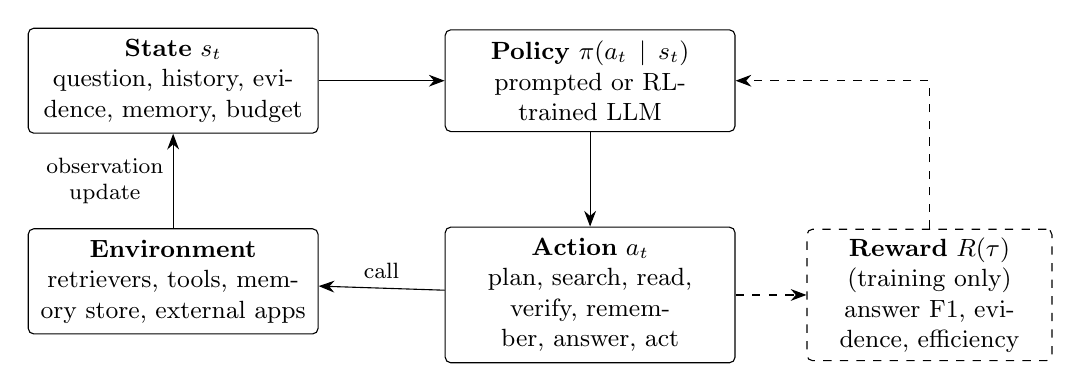
\begin{tikzpicture}[
  font=\small,
  box/.style={draw, rounded corners=2pt, align=center, inner sep=4pt, minimum height=9mm, text width=3.4cm},
  side/.style={draw, dashed, rounded corners=2pt, align=center, inner sep=3pt, text width=2.9cm},
  arr/.style={-{Stealth[length=2mm]}}
]
\node[box] (state) {\textbf{State} $s_t$\\question, history, evidence, memory, budget};
\node[box, right=1.6cm of state] (policy) {\textbf{Policy} $\pi(a_t \mid s_t)$\\prompted or RL-trained LLM};
\node[box, below=1.2cm of policy] (act) {\textbf{Action} $a_t$\\plan, search, read, verify, remember, answer, act};
\node[box, below=1.2cm of state] (env) {\textbf{Environment}\\retrievers, tools, memory store, external apps};
\node[side, right=0.9cm of act] (reward) {\textbf{Reward} $R(\tau)$ (training only)\\answer F1, evidence, efficiency};
\draw[arr] (state) -- (policy);
\draw[arr] (policy) -- (act);
\draw[arr] (act) -- node[above, font=\footnotesize] {call} (env);
\draw[arr] (env) -- node[left, font=\footnotesize, align=center] {observation\\update} (state);
\draw[arr, dashed] (act) -- (reward);
\draw[arr, dashed] (reward) |- (policy);
\end{tikzpicture}%
}
\caption{The decision loop shared by agentic RAG methods. Each design dimension of Fig.~\ref{fig:taxonomy} corresponds to a part of this loop that a method hands to the model: which actions exist, how the policy is obtained, what the state keeps, and what the reward measures.}
\label{fig:loop}
\end{figure}

Seen this way, the methods in this survey differ along a small number of axes: which actions exist (only ``search'', or also ``read more'', ``verify'' and ``remember''), how the policy is obtained (prompting, a trained classifier, supervised fine-tuning or RL), what the state carries across turns and across sessions, and what the reward, if any, measures. These axes give the taxonomy in the next section.

%=====================================================================
\section{A Taxonomy of Agentic RAG}
\label{sec:taxonomy}
%=====================================================================

Fig.~\ref{fig:taxonomy} groups the literature into eight dimensions. A single system usually makes choices along several of them at once; the figure lists each method where its main contribution lies.

\begin{figure*}[t]
\centering
\resizebox{\textwidth}{!}{%
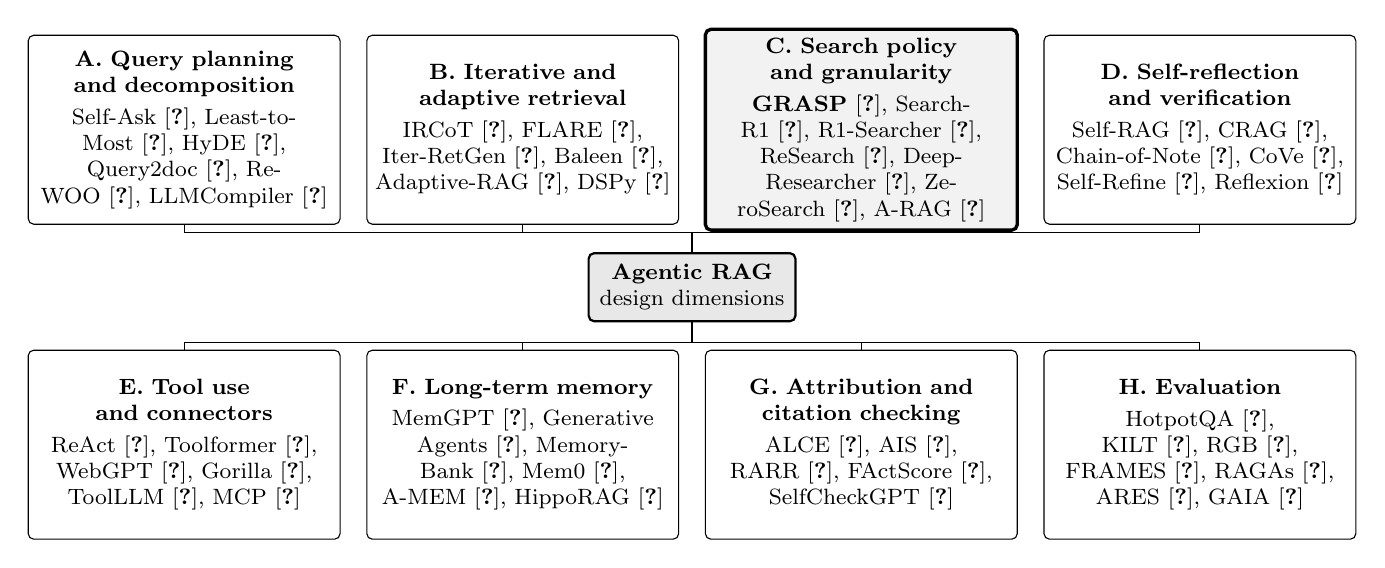
\begin{tikzpicture}[
  font=\footnotesize,
  root/.style={draw, thick, rounded corners=2pt, fill=gray!18, align=center, inner sep=4pt, minimum height=7mm},
  cat/.style={draw, rounded corners=2pt, align=center, text width=3.75cm, minimum height=2.4cm, inner sep=3pt},
  hl/.style={cat, very thick, fill=gray!10}
]
\node[root] (root) at (0,0) {\textbf{Agentic RAG}\\design dimensions};
\node[cat] (a) at (-6.45, 2.0) {\textbf{A. Query planning and decomposition}\\[2pt] Self-Ask~\cite{press2023selfask}, Least-to-Most~\cite{zhou2023leasttomost}, HyDE~\cite{gao2023hyde}, Query2doc~\cite{wang2023query2doc}, ReWOO~\cite{xu2023rewoo}, LLMCompiler~\cite{kim2024llmcompiler}};
\node[cat] (b) at (-2.15, 2.0) {\textbf{B. Iterative and adaptive retrieval}\\[2pt] IRCoT~\cite{trivedi2023ircot}, FLARE~\cite{jiang2023flare}, Iter-RetGen~\cite{shao2023iterretgen}, Baleen~\cite{khattab2021baleen}, Adaptive-RAG~\cite{jeong2024adaptiverag}, DSPy~\cite{khattab2024dspy}};
\node[hl]  (c) at ( 2.15, 2.0) {\textbf{C. Search policy and granularity}\\[2pt] \textbf{GRASP}~\cite{gandhi2026grasp}, Search-R1~\cite{jin2025searchr1}, R1-Searcher~\cite{song2025r1searcher}, ReSearch~\cite{chen2025research}, DeepResearcher~\cite{zheng2025deepresearcher}, ZeroSearch~\cite{sun2025zerosearch}, A-RAG~\cite{du2026arag}};
\node[cat] (d) at ( 6.45, 2.0) {\textbf{D. Self-reflection and verification}\\[2pt] Self-RAG~\cite{asai2024selfrag}, CRAG~\cite{yan2024crag}, Chain-of-Note~\cite{yu2024chainofnote}, CoVe~\cite{dhuliawala2024cove}, Self-Refine~\cite{madaan2023selfrefine}, Reflexion~\cite{shinn2023reflexion}};
\node[cat] (e) at (-6.45,-2.0) {\textbf{E. Tool use and connectors}\\[2pt] ReAct~\cite{yao2023react}, Toolformer~\cite{schick2023toolformer}, WebGPT~\cite{nakano2021webgpt}, Gorilla~\cite{patil2024gorilla}, ToolLLM~\cite{qin2024toolllm}, MCP~\cite{anthropic2024mcp}};
\node[cat] (f) at (-2.15,-2.0) {\textbf{F. Long-term memory}\\[2pt] MemGPT~\cite{packer2023memgpt}, Generative Agents~\cite{park2023generative}, MemoryBank~\cite{zhong2024memorybank}, Mem0~\cite{chhikara2025mem0}, A-MEM~\cite{xu2025amem}, HippoRAG~\cite{gutierrez2024hipporag}};
\node[cat] (g) at ( 2.15,-2.0) {\textbf{G. Attribution and citation checking}\\[2pt] ALCE~\cite{gao2023alce}, AIS~\cite{rashkin2023ais}, RARR~\cite{gao2023rarr}, FActScore~\cite{min2023factscore}, SelfCheckGPT~\cite{manakul2023selfcheckgpt}};
\node[cat] (h) at ( 6.45,-2.0) {\textbf{H. Evaluation}\\[2pt] HotpotQA~\cite{yang2018hotpotqa}, KILT~\cite{petroni2021kilt}, RGB~\cite{chen2024rgb}, FRAMES~\cite{krishna2025frames}, RAGAs~\cite{es2024ragas}, ARES~\cite{saadfalcon2024ares}, GAIA~\cite{mialon2024gaia}};
\draw (root.north) -- (0,0.7);
\draw (-6.45,0.7) -- (6.45,0.7);
\foreach \nd/\x in {a/-6.45,b/-2.15,c/2.15,d/6.45} { \draw (\x,0.7) -- (\nd.south); }
\draw (root.south) -- (0,-0.7);
\draw (-6.45,-0.7) -- (6.45,-0.7);
\foreach \nd/\x in {e/-6.45,f/-2.15,g/2.15,h/6.45} { \draw (\x,-0.7) -- (\nd.north); }
\end{tikzpicture}%
}
\caption{The eight design dimensions used in this survey, with representative (not exhaustive) methods for each. Dimension C, shaded, holds the RL-trained search policies, including GRASP~\cite{gandhi2026grasp}, which Section~\ref{sec:grasp} examines in detail.}
\label{fig:taxonomy}
\end{figure*}

%---------------------------------------------------------------------
\subsection{Query Planning and Decomposition}
\label{sec:planning}
A question that needs several facts can be broken up before any search runs. Chain-of-thought prompting showed that writing out intermediate steps improves multi-step reasoning~\cite{wei2022cot}, and least-to-most prompting made the split explicit: solve easy subproblems first and feed their answers into harder ones~\cite{zhou2023leasttomost}. Self-Ask applies this to retrieval, generating follow-up questions and sending each to a search engine~\cite{press2023selfask}.

A second group rewrites the query rather than splitting it. HyDE has an LLM write a hypothetical answer document and retrieves real documents near its embedding~\cite{gao2023hyde}. Query2doc appends such a pseudo-document to the query and reports gains of 3--15\% for BM25 on MS MARCO and TREC DL without any fine-tuning~\cite{wang2023query2doc}. Rewrite-Retrieve-Read trains a small rewriter with RL, using the reader's success as the reward~\cite{ma2023rewrite}.

The third group concerns \emph{when} the plan is made. ReAct decides each action only after seeing the previous observation~\cite{yao2023react}. ReWOO separates planning from observation: it writes the whole plan with placeholders for tool outputs, runs the tools, and only then reasons over the results, which cuts token use substantially~\cite{xu2023rewoo}. LLMCompiler goes further and compiles the plan into a dependency graph whose independent calls run in parallel~\cite{kim2024llmcompiler}. The same trade-off appears in all three papers. A plan written up front uses fewer tokens and its calls can run in parallel. A plan built step by step can react to what it finds, and multi-hop questions need that, because the next query depends on the last answer.

%---------------------------------------------------------------------
\subsection{Iterative and Adaptive Retrieval}
Iterative methods retrieve during generation rather than before it. IRCoT uses each new chain-of-thought sentence as the next query, so retrieval follows the reasoning~\cite{trivedi2023ircot}. FLARE drafts the next sentence and retrieves only if the draft contains low-confidence tokens~\cite{jiang2023flare}. Iter-RetGen alternates between retrieval and generation, using the whole draft answer as the next query~\cite{shao2023iterretgen}. Baleen, an earlier multi-hop retriever, summarises what each hop found into one condensed context before the next hop, which keeps the search space under control across many hops~\cite{khattab2021baleen}.

Adaptive methods decide \emph{whether} and \emph{how much} to retrieve. Adaptive-RAG trains a small classifier that sends each question to no retrieval, single-step retrieval or multi-step retrieval according to its predicted complexity~\cite{jeong2024adaptiverag}, and Self-Route makes the same kind of choice between RAG and a long context~\cite{li2024ragvslc}. DSPy treats such pipelines as programs: modules declare what they do, and a compiler optimises prompts and demonstrations for a target metric instead of a human tuning them by hand~\cite{khattab2024dspy}. All of these vary when retrieval happens or which pipeline runs; the retriever and the size of the text unit stay fixed.

%---------------------------------------------------------------------
\subsection{Learned Search Policies and Evidence Granularity}
\label{sec:policies}
The most active part of the field since 2025 trains the search loop itself with RL, encouraged by the finding that RL alone can teach long chains of reasoning~\cite{deepseek2025r1} and by group-relative policy optimisation (GRPO), which removes the need for a separate value model~\cite{shao2024deepseekmath}. Search-R1 trains a model to issue search calls inside its reasoning and rewards only the final answer~\cite{jin2025searchr1}. R1-Searcher uses a two-stage, outcome-based RL scheme and needs neither process rewards nor a distilled cold start~\cite{song2025r1searcher}. ReSearch treats search as part of the reasoning chain, trains Qwen2.5 models of 7B and 32B parameters on a single dataset, and reports that the learned behaviour transfers to other benchmarks~\cite{chen2025research}. Search-o1 adds agentic search to large reasoning models at inference time~\cite{li2025searcho1}.

These methods train against a fixed local corpus. Two papers question that setting from opposite sides. DeepResearcher trains in the real web, arguing that a fixed corpus that is known to contain the answer hides the noise and dead ends of real search~\cite{zheng2025deepresearcher}. ZeroSearch argues that live search is too costly and too erratic for RL, which needs very many rollouts, and replaces the search engine during training with an LLM that simulates one~\cite{sun2025zerosearch}. Both are trying to make the training environment look more like deployment without paying deployment's price.

A third set of methods widens the action set. MARAG-R1 gives an agent semantic, keyword, filter and aggregation tools and trains it with supervised fine-tuning followed by RL~\cite{luo2025maragr1}. A-RAG exposes keyword search, semantic search and chunk reading as separate, hierarchical interfaces that a model calls directly~\cite{du2026arag}. GRASP adds the one action the others lack: the choice of how much to read~\cite{gandhi2026grasp}.

\subsubsection{GRASP in depth}
\label{sec:grasp}
\paragraph{Problem.} Gandhi \textit{et al.} note that RL-trained retrieval agents are usually tied to one retriever and to fixed chunks of moderate size~\cite{gandhi2026grasp}. The kind and amount of evidence cannot then change from one step to the next. GRASP (GRanularity-Aware Search Policy) learns three decisions in one policy: how to mix lexical and dense search, how much to read, and when to stop.

\paragraph{Formulation and actions.} The search loop is a Markov decision process with a fixed turn limit. The state holds the question, the history, the evidence and tools used so far, and the remaining budget. Every paragraph is split into sentences that keep a pointer to it. At each step the policy reasons and then takes one action: \emph{semantic search} (Qwen3-0.6B embeddings), \emph{keyword search} (BM25), \emph{read paragraph} (the parent of a retrieved sentence) or \emph{answer}. Searches return the top $K=5$ sentences, so a full paragraph costs context only when the agent asks for it.

\paragraph{Reward.} The trajectory reward is
\begin{equation}
R = R_A + \alpha R_R + \beta R_S + \gamma R_E, \qquad (\alpha,\beta,\gamma) = (0.7,\, 0.15,\, 0.15).
\label{eq:grasp}
\end{equation}
$R_A$ is the token-level F1 of the answer. $R_R$ is the F1 between the paragraphs the agent read and the gold supporting paragraphs, which penalises reading distractors. $R_S$ is 1 only if semantic and keyword search \emph{each} found a gold paragraph, which pushes the agent to use both. $R_E = (T - T_{\mathrm{cur}})/T$, with $T$ the turn budget, rewards finishing early, but it is paid only when $R_A > 0.5$, so a fast wrong answer earns nothing. The auxiliary weights sum to one, which keeps answer F1 dominant and limits reward hacking.

\paragraph{Training and evaluation.} Qwen2.5-3B-Instruct is trained with GRPO~\cite{shao2024deepseekmath} on the HotpotQA distractor split~\cite{yang2018hotpotqa} for 270 steps, about 19\% of one epoch. Episodes end after 10 turns, and retrieved tokens are masked out of the loss. The test sets are 500 validation questions from each of HotpotQA, 2WikiMultiHopQA and MuSiQue~\cite{yang2018hotpotqa,ho2020twowiki,trivedi2022musique}; the last two are never seen in training. Baselines include single-step lexical, semantic and hybrid retrieval, IRCoT driven by a proprietary model, the public Search-R1 checkpoints trained with PPO and GRPO, and an untrained ``Base'' agent with GRASP's prompt and tools.

\begin{table}[t]
\centering
\caption{Results reported by GRASP~\cite{gandhi2026grasp}: retrieval recall (R) and answer F1 on 500 validation questions per dataset. GRASP has the best F1 on all three, while IRCoT leads on HotpotQA recall. Numbers are copied from the GRASP paper, not re-run.}
\label{tab:grasp}
\setlength{\tabcolsep}{4pt}
\footnotesize
\begin{tabular}{@{}lcccccc@{}}
\toprule
 & \multicolumn{2}{c}{HotpotQA} & \multicolumn{2}{c}{2Wiki} & \multicolumn{2}{c}{MuSiQue} \\
\cmidrule(lr){2-3}\cmidrule(lr){4-5}\cmidrule(lr){6-7}
Method & R & F1 & R & F1 & R & F1 \\
\midrule
Single-step hybrid   & 0.86 & 0.48 & 0.60 & 0.32 & 0.59 & 0.20 \\
IRCoT                & \textbf{0.91} & 0.36 & 0.83 & 0.40 & 0.62 & 0.15 \\
Search-R1 (PPO)      & 0.76 & 0.47 & 0.74 & 0.48 & 0.55 & 0.26 \\
Search-R1 (GRPO)     & 0.74 & 0.56 & 0.77 & 0.53 & 0.62 & 0.30 \\
Base (no RL)         & 0.36 & 0.24 & 0.27 & 0.20 & 0.24 & 0.10 \\
GRASP                & 0.90 & \textbf{0.66} & \textbf{0.90} & \textbf{0.60} & \textbf{0.70} & \textbf{0.33} \\
\bottomrule
\end{tabular}
\end{table}

\paragraph{Findings.} GRASP has the best F1 on all three datasets and the best recall on 2WikiMultiHopQA and MuSiQue (Table~\ref{tab:grasp}). The authors attribute IRCoT's slightly higher HotpotQA recall to the strong proprietary model that writes its reasoning. Even single-step retrieval beats the untrained Base agent, so tools do little for a model that has not learned to use them. The ablation is the most informative result. On HotpotQA, removing keyword search lowers F1 only from 0.631 to 0.621 and removing semantic search lowers it to 0.567, but removing the read action, so that searches return whole paragraphs, drops it to 0.484. The authors' explanation is that a paragraph shows many entities at once, and the agent's next queries drift back towards the original question instead of following a single clue. A typical learned trajectory starts with a semantic search, reads one paragraph to pick up a bridge entity, runs a keyword search on that entity, and falls back to a broader semantic query if the keyword search fails.

\paragraph{Limitations.} $R_R$ and $R_S$ need gold supporting facts, which few real corpora have. The policy sometimes answers too early, tool use levels off at about eight calls, and only one 3B backbone was tested. The authors propose larger tool sets, rewards built from weaker or model-based grounding signals, and units that range from spans to whole document regions. Their ethics statement recommends provenance, citations, audit logs and human approval for consequential actions, points that return in Section~\ref{sec:security}.

\paragraph{What GRASP adds to the picture.} Search-R1, R1-Searcher and ReSearch learn \emph{when} and \emph{what} to search. GRASP also learns \emph{how much to read}, and on HotpotQA its ablation finds that removing this choice costs more F1 than removing either retriever. That is the same tension Dense X and LongRAG resolve in opposite directions at index time~\cite{chen2024densex,jiang2024longrag}; GRASP resolves it per step.

%---------------------------------------------------------------------
\subsection{Self-Reflection, Correction and Verification}
A second family checks evidence or answers rather than searching better. Self-RAG fine-tunes a model to emit reflection tokens that decide whether to retrieve and grade each passage for relevance and support~\cite{asai2024selfrag}. CRAG scores what was retrieved with a lightweight evaluator and falls back to web search when the documents look poor~\cite{yan2024crag}. Chain-of-Note has the model write a short reading note on each retrieved document before answering, and to answer ``unknown'' when neither the documents nor its own knowledge suffice~\cite{yu2024chainofnote}.

Other methods correct the answer after it is written. Self-Refine has one model draft, critique and revise its own output, with no training~\cite{madaan2023selfrefine}. Chain-of-Verification (CoVe) drafts an answer, plans verification questions about it, answers those questions independently so that the draft cannot bias them, and then writes a revised answer~\cite{dhuliawala2024cove}. Reflexion stores written lessons from failed attempts for the next try~\cite{shinn2023reflexion}. GRASP has no critic at inference time; its grounded-reading reward plays that role, but only during training. An open question this raises is whether a verifier at inference time and a grounding term in the reward are substitutes or complements; we found no study that tests both on the same policy.

%---------------------------------------------------------------------
\subsection{Tool Use and Connector Protocols}
Retrieval is one tool among many once a model can call functions. WebGPT trained GPT-3 to browse with a text-based browser, collecting references as it went; its answers were preferred to those of the human demonstrators 56\% of the time~\cite{nakano2021webgpt}. ReAct made interleaved reasoning and tool calls the default pattern~\cite{yao2023react}. Toolformer taught a model from a few demonstrations where an API call helps~\cite{schick2023toolformer}, Gorilla fine-tuned a model to write accurate API calls and paired it with a retriever over API documentation so it can follow documentation changes at test time~\cite{patil2024gorilla}, and ToolLLM built ToolBench from 16,464 real REST APIs in 49 categories~\cite{qin2024toolllm}.

The Model Context Protocol (MCP), released by Anthropic in November 2024, standardises how clients discover and call external tools and data sources~\cite{anthropic2024mcp}. It makes it much easier to connect an agent to private systems such as mail, calendars and code hosts, and each new connection is also a new point of attack~\cite{hou2025mcp}; Section~\ref{sec:security} returns to this.

%---------------------------------------------------------------------
\subsection{Long-Term Memory}
Retrieval over a fixed corpus answers ``what does the collection say''; memory answers ``what has this user told me before''. MemGPT pages information between the context window and external storage much as an operating system pages memory~\cite{packer2023memgpt}. Generative Agents score each memory by recency, importance and relevance and periodically write higher-level reflections~\cite{park2023generative}. MemoryBank updates and forgets memories along the Ebbinghaus forgetting curve~\cite{zhong2024memorybank}. Mem0 extracts and consolidates salient facts from conversations, with an optional graph variant~\cite{chhikara2025mem0}, and A-MEM organises memories as linked notes in the style of the Zettelkasten method, letting new memories update old ones~\cite{xu2025amem}. HippoRAG, discussed above as a retriever, is also framed by its authors as long-term memory that integrates new experience after pre-training~\cite{gutierrez2024hipporag}.

Evaluation lags behind. LongMemEval tests five abilities, information extraction, multi-session reasoning, temporal reasoning, knowledge updates and abstention, on 500 questions, and reports a 30\% accuracy drop for commercial assistants and long-context models over sustained interactions~\cite{wu2025longmemeval}. Once memory holds personal data, its provenance, expiry and deletion become design requirements rather than afterthoughts, and none of the benchmarks above measures them.

%---------------------------------------------------------------------
\subsection{Attribution and Citation Checking}
An answer that cites its sources can still misrepresent them. ALCE measures whether cited passages actually support each statement and finds that, often, they do not~\cite{gao2023alce}. AIS defines attribution to identified sources as a rating task for humans~\cite{rashkin2023ais}. FActScore splits a generation into atomic facts and scores each against a knowledge source~\cite{min2023factscore}. RARR works after the fact: it finds evidence for a model's output and post-edits unsupported content while keeping the rest~\cite{gao2023rarr}. SelfCheckGPT needs no external source at all, flagging statements that vary across several sampled answers as likely hallucinations~\cite{manakul2023selfcheckgpt}. These methods score individual claims, which makes them a natural source of the weaker, model-based grounding signal that GRASP lists as future work; Section~\ref{sec:challenges} discusses the risk in that idea.

%=====================================================================
\section{Comparative Analysis}
\label{sec:compare}
%=====================================================================

Table~\ref{tab:compare} codes 25 representative methods along the taxonomy. ``Granularity'' records whether the evidence unit is fixed in advance or chosen by the agent, and ``Live data'' whether the sources can change while the agent runs. A dash means the method does not address that dimension in its publication.

\begin{table*}[t]
\centering
\caption{Representative methods along the taxonomy dimensions, as described in each publication. Reading down the columns shows which decisions are rarely combined: no RL-trained search policy also keeps long-term memory or takes actions in external systems.}
\label{tab:compare}
\scriptsize
\setlength{\tabcolsep}{3pt}
\renewcommand{\arraystretch}{1.1}
\resizebox{\textwidth}{!}{%
\begin{tabular}{@{}L{2.8cm}L{3.1cm}L{2.1cm}L{2.2cm}L{1.7cm}L{2.4cm}L{1.6cm}L{1.6cm}@{}}
\toprule
\textbf{Method} & \textbf{Retrieval strategy} & \textbf{Granularity} & \textbf{Policy} & \textbf{Memory} & \textbf{Verification} & \textbf{Live data} & \textbf{Actions} \\
\midrule
RAG~\cite{lewis2020rag} & Single-shot dense retrieval & Fixed passage & Fine-tuned retriever, generator & -- & -- & -- & -- \\
REPLUG~\cite{shi2024replug} & Prepend to black-box LM & Fixed passage & LM-supervised retriever & -- & -- & -- & -- \\
Self-Ask~\cite{press2023selfask} & Follow-up sub-questions & Search-engine answer & Prompting & -- & -- & Web search & -- \\
ReWOO~\cite{xu2023rewoo} & Plan first, then call tools & Tool output & Prompting & -- & -- & Tools & -- \\
LLMCompiler~\cite{kim2024llmcompiler} & Parallel tool-call graph & Tool output & Prompting (planner) & -- & -- & Tools & Function calls \\
IRCoT~\cite{trivedi2023ircot} & Retrieve at each reasoning step & Fixed paragraph & Prompting & -- & -- & -- & -- \\
FLARE~\cite{jiang2023flare} & Retrieve on low confidence & Fixed passage & Prompting & -- & Regenerate uncertain sentence & -- & -- \\
Adaptive-RAG~\cite{jeong2024adaptiverag} & None, single or multi-step & Fixed & Trained classifier & -- & -- & -- & -- \\
HippoRAG~\cite{gutierrez2024hipporag} & PageRank over LLM-built graph & Passage via graph & Fixed algorithm & Graph index & -- & -- & -- \\
Self-RAG~\cite{asai2024selfrag} & On demand, reflection tokens & Fixed passage & Fine-tuned & -- & Relevance, support tokens & -- & -- \\
CRAG~\cite{yan2024crag} & Evaluator-triggered correction & Strip filtering & Trained evaluator & -- & Retrieval evaluator & Web fallback & -- \\
Chain-of-Note~\cite{yu2024chainofnote} & Notes on each document & Fixed passage & Fine-tuned & -- & Reading notes, ``unknown'' & -- & -- \\
CoVe~\cite{dhuliawala2024cove} & Answer, then verify & -- & Prompting & -- & Independent verification questions & -- & -- \\
ReAct~\cite{yao2023react} & Interleaved thought and action & API page or lookup & Prompting & -- & -- & Wikipedia API & Environment actions \\
WebGPT~\cite{nakano2021webgpt} & Text-based browsing & Quoted spans & Imitation, then RLHF & -- & Collected references & Live web & Browser commands \\
Search-R1~\cite{jin2025searchr1} & Search inside reasoning & Fixed passage & RL (PPO, GRPO) & -- & -- & -- & -- \\
R1-Searcher~\cite{song2025r1searcher} & Search inside reasoning & Fixed passage & Two-stage outcome RL & -- & -- & -- & -- \\
ReSearch~\cite{chen2025research} & Search as reasoning step & Fixed passage & RL, no step labels & -- & -- & -- & -- \\
DeepResearcher~\cite{zheng2025deepresearcher} & Multi-step web research & Web page & RL in the real web & -- & -- & Live web & Browsing \\
ZeroSearch~\cite{sun2025zerosearch} & Search inside reasoning & Simulated documents & RL with simulated search & -- & -- & -- & -- \\
MARAG-R1~\cite{luo2025maragr1} & Semantic, keyword, filter, aggregate & Fixed chunk & SFT, then RL & -- & -- & -- & -- \\
A-RAG~\cite{du2026arag} & Hierarchical retrieval interfaces & Keyword to chunk & Model-driven tool use & -- & -- & -- & -- \\
\textbf{GRASP}~\cite{gandhi2026grasp} & Coordinated semantic and keyword & Sentence; paragraph on demand & RL (GRPO), 4-part reward & -- & Grounded reading (training only) & -- & -- \\
MemGPT~\cite{packer2023memgpt} & Paging context and storage & -- & Function calls & Tiered context & -- & -- & -- \\
A-MEM~\cite{xu2025amem} & Linked-note retrieval & Note & Prompting & Evolving note graph & -- & -- & -- \\
\bottomrule
\end{tabular}%
}
\end{table*}

Four patterns follow from the table.

\textbf{Learned policies live in static worlds.} Every RL-trained search policy except DeepResearcher is trained and tested on a fixed, mostly Wikipedia-based corpus in which the answer is known to exist, and the strongest auxiliary rewards (GRASP's $R_R$ and $R_S$) need gold supporting facts. Methods that query live sources (Self-Ask, ReAct, WebGPT, CRAG's fallback) mostly rely on prompting. ZeroSearch's simulated search engine and DeepResearcher's real one are the two attempts we found to close this gap, and they pull in opposite directions on cost and realism.

\textbf{Granularity is rarely a decision.} Only A-RAG and GRASP let the agent choose the evidence unit at query time. Index-time choices (propositions, long units, summary trees, graphs) are common, and the evidence from Dense X, LongRAG and GRASP's ablation together suggests the right unit depends on the question, which is an argument for making it a per-step choice.

\textbf{Verification and retrieval are studied apart.} Methods with explicit verification (Self-RAG, CRAG, Chain-of-Note, CoVe) use fixed retrieval; methods with learned retrieval have no verifier at inference time. The two families answer different halves of the same problem, finding evidence and judging it, and the table contains no method that learns both.

\textbf{Memory and actions are absent from learned retrieval.} Long-term memory appears only in memory-specific systems, and side-effecting actions only in prompted tool agents and in DeepResearcher's browsing. No method in the table combines an RL-trained search policy with persistent memory or with actions in external systems, although deployed assistants need all three.

%=====================================================================
\section{Benchmarks and Evaluation}
\label{sec:eval}
%=====================================================================

Table~\ref{tab:bench} summarises the benchmarks used by the surveyed work and what each one tests.

\begin{table}[t]
\centering
\caption{Benchmarks for retrieval agents and what each one measures. Sizes are as reported by the benchmark authors where they state one.}
\label{tab:bench}
\scriptsize
\setlength{\tabcolsep}{3pt}
\renewcommand{\arraystretch}{1.1}
\begin{tabular}{@{}L{2.9cm}L{2.7cm}L{5.4cm}@{}}
\toprule
\textbf{Benchmark} & \textbf{Setting} & \textbf{What it tests} \\
\midrule
HotpotQA, 2Wiki, MuSiQue~\cite{yang2018hotpotqa,ho2020twowiki,trivedi2022musique} & Wikipedia, multi-hop & Bridge and comparison questions; gold supporting facts \\
KILT~\cite{petroni2021kilt} & One Wikipedia snapshot & Several knowledge tasks; provenance of answers \\
BEIR~\cite{thakur2021beir} & 18 retrieval datasets & Zero-shot retrieval across domains \\
RGB~\cite{chen2024rgb} & English and Chinese & Noise, negative rejection, integration, counterfactuals \\
MultiHop-RAG~\cite{tang2024multihoprag} & News articles & Multi-hop queries over a realistic knowledge base \\
FRAMES~\cite{krishna2025frames} & 824 questions & Factuality, retrieval and reasoning together \\
FreshQA~\cite{vu2024freshllms} & Changing facts & Answers whose truth changes over time \\
RAGAs, ARES~\cite{es2024ragas,saadfalcon2024ares} & Any RAG system & Faithfulness and relevance without full references \\
GAIA~\cite{mialon2024gaia} & Assistant tasks & Reasoning, browsing, tool use (humans 92\%, GPT-4 with plugins 15\%) \\
BrowseComp~\cite{wei2025browsecomp} & 1,266 web questions & Persistent search for hard-to-find facts \\
AgentBench~\cite{liu2024agentbench} & 8 environments & General LLM-as-agent decision-making \\
LongMemEval~\cite{wu2025longmemeval} & 500 questions & Five long-term memory abilities in chat \\
\bottomrule
\end{tabular}
\end{table}

Most agentic RAG work, GRASP included, reports results on the three Wikipedia multi-hop datasets. They are well understood and provide gold evidence, which RL rewards need, but they share three properties that real deployments lack: one clean source, facts that do not change, and no actions. Newer benchmarks address one property each. MultiHop-RAG moves to news~\cite{tang2024multihoprag}; FreshQA targets facts that change~\cite{vu2024freshllms}; FRAMES evaluates retrieval and reasoning together instead of in isolation~\cite{krishna2025frames}; GAIA and BrowseComp score agents that browse and use tools~\cite{mialon2024gaia,wei2025browsecomp}. Reference-free scorers such as RAGAs and ARES make evaluation cheaper; ARES fine-tunes small judges on synthetic data and corrects them with a few hundred human labels~\cite{es2024ragas,saadfalcon2024ares}.

What is missing is a benchmark that combines the properties. We found none in which an agent answers from private, heterogeneous sources (mail, chat, documents, code), those sources change during the evaluation, answers must cite and be checked against evidence, honest abstention counts as success, conflicts between sources must be surfaced, and some tasks require an action whose safety is scored. Each of these appears somewhere in Table~\ref{tab:bench}, but never together.

%=====================================================================
\section{Security and Robustness}
\label{sec:security}
%=====================================================================

Giving a model control over retrieval also gives an attacker more ways in. Three threats recur in the surveyed work.

\textbf{Indirect prompt injection.} Text that the agent retrieves can contain instructions, and the model may follow them~\cite{greshake2023injection}. The risk grows with each tool an agent can call. InjecAgent measures it with 1,054 test cases spanning 17 user tools and 62 attacker tools, separating direct harm to the user from exfiltration of private data~\cite{zhan2024injecagent}. AgentDojo provides 97 realistic tasks, such as managing an email client or making travel bookings, with 629 security test cases, and is built as an extensible environment so that new attacks and defences can be added~\cite{debenedetti2024agentdojo}.

\textbf{Knowledge corruption.} PoisonedRAG shows that injecting a few malicious texts into the knowledge base can steer a RAG system to an attacker-chosen answer for a target question~\cite{zou2025poisonedrag}. For an agent that searches repeatedly, each search is another chance to retrieve poisoned text.

\textbf{Connector and protocol risk.} Protocols such as MCP make it easy to attach many tools to one agent~\cite{anthropic2024mcp}, and every server added is code and data the agent trusts~\cite{hou2025mcp}.

The defences in the literature are partial. Approval gates, under which consequential actions run only after a human confirms an exact preview, limit the damage an injected instruction can do; GRASP's authors recommend human approval for consequential actions for this reason~\cite{gandhi2026grasp}. Separating retrieved data from instructions, provenance on every piece of evidence, and audit logs reduce the risk further. None of these removes it, and the AgentDojo authors report that their environment remains a challenge for attacks and defences alike~\cite{debenedetti2024agentdojo}.

%=====================================================================
\section{Open Challenges and Future Directions}
\label{sec:challenges}
%=====================================================================

\textbf{Supervision without gold evidence.} The richest RL rewards need gold supporting facts~\cite{gandhi2026grasp,luo2025maragr1}, which private corpora do not have. Claim-level scores of the AIS or FActScore kind~\cite{rashkin2023ais,min2023factscore}, verifier labels, and agreement across sampled trajectories~\cite{manakul2023selfcheckgpt} are candidate substitutes. Each brings a risk: a policy rewarded by a partly lexical or model-based checker can learn to satisfy the checker rather than the user. Human spot checks, and rewards that combine several weak signals, are the obvious safeguards; we found no study that measures how much reward gaming they prevent.

\textbf{Evidence units for heterogeneous data.} GRASP's sentence-and-paragraph pair has no obvious counterpart in an email thread, a pull request, a calendar event or a chat channel. Hierarchical units~\cite{sarthi2024raptor,du2026arag}, propositions~\cite{chen2024densex}, long units~\cite{jiang2024longrag} and graphs~\cite{edge2024graphrag,gutierrez2024hipporag} give starting points, but the right ``read more'' action probably differs by source.

\textbf{Learning retrieval and verification together.} The comparison in Section~\ref{sec:compare} shows the two developing separately. A policy that searches, judges its evidence with a learned critic, and decides to search again when the critic disagrees would join the strengths of the GRASP and Self-RAG families.

\textbf{Freshness and conflict.} Time-sensitive questions remain hard~\cite{vu2024freshllms}, and most methods treat conflicting evidence as noise to filter. When sources disagree, for example two documents giving different deadlines, a useful agent should show the disagreement and its sources rather than pick a side silently.

\textbf{Memory governance.} Memory systems~\cite{packer2023memgpt,zhong2024memorybank,chhikara2025mem0,xu2025amem} raise questions that benchmarks such as LongMemEval do not yet measure: whether the user can see why something was remembered, whether stale memories expire, and whether deletion is complete.

\textbf{Safety of acting agents.} Prompt injection and knowledge corruption remain open~\cite{zhan2024injecagent,debenedetti2024agentdojo,zou2025poisonedrag}. Approval gates help, but they move the burden to the user; methods that reduce how often a user must approve, without raising risk, are needed.

\textbf{Cost-aware evaluation.} GRASP settles at about eight tool calls~\cite{gandhi2026grasp}, and LLMCompiler and ReWOO show how much latency and token cost depend on the plan~\cite{kim2024llmcompiler,xu2023rewoo}. Benchmarks should report cost alongside accuracy, and should credit citation support, honest abstention, conflict reporting and action safety, not answer accuracy alone.

%=====================================================================
\section{Conclusion}
\label{sec:conclusion}
%=====================================================================

Agentic RAG turns retrieval from a fixed preprocessing step into a sequence of decisions made by the model. Framed as a decision problem, the literature splits into eight dimensions. Each dimension has made progress on its own, but few methods combine them. RL-trained search policies such as Search-R1, R1-Searcher, ReSearch and GRASP now learn when and what to search, and GRASP's ablation on HotpotQA suggests that learning how much to read matters more than which retriever is used. Verification, memory and safe action have their own strong methods. Yet the learned policies are trained on static corpora with gold evidence, none of them verifies at inference time or keeps memory, and no benchmark tests an agent over private, changing data that it can also act on. Closing those gaps needs rewards that do not depend on gold evidence, evidence units suited to mail, chat and code, joint training of retrieval and verification, and evaluations that score trust and safety alongside accuracy.

%=====================================================================
\section*{Threats to Validity}
%=====================================================================
The survey covers work found through the search described in Section~\ref{sec:method}; relevant systems outside those sources, or published after the search, may be missing. Several recent works, including some of the RL-trained search policies, were available only as preprints at the time of writing, and all reported numbers are reproduced from the original papers rather than re-run. The coding of methods in Table~\ref{tab:compare} reflects what each publication describes and may understate capabilities that a method has but does not report.

\backmatter

\section*{Declarations}

\begin{itemize}
\item \textbf{Funding:} No funding was received for this study.
\item \textbf{Conflict of interest:} On behalf of all authors, the corresponding author states that there is no conflict of interest.
\item \textbf{Ethics approval:} Not applicable; this is a literature review with no human participants or data.
\item \textbf{Data availability:} No new data were generated or analysed. All results discussed are taken from the cited publications.
\item \textbf{Author contributions:} All authors contributed to the literature search, analysis and writing of the manuscript. S.G.\ supervised the work. All authors read and approved the final manuscript.
\item \textbf{Use of generative AI:} An AI assistant was used to help structure the manuscript, to draft and edit sections based on the authors' earlier conference paper and notes, and for reference management. All AI-assisted text was reviewed and revised by the authors, every reference was checked against the original source, and the authors take full responsibility for the content.
\end{itemize}

\bibliography{refs}

\end{document}
